\documentclass[a4paper]{article}
\usepackage[paperwidth=17cm, paperheight=22.5cm, bottom=2.5cm, right=2.5cm]{geometry}
\setlength{\parindent}{2cm}
\setlength{\parskip}{\baselineskip}
\setlength{\parindent}{0pt}
\usepackage[utf8x]{inputenc}
\usepackage{verbatim} % comentarios
\usepackage{pdfpages}

\usepackage[spanish]{babel}
%% Useful packages
\usepackage{amsmath}
\usepackage{amssymb}
\usepackage[hidelinks]{hyperref}
\usepackage{listings}
\usepackage{graphicx}

%\usepackage{subfig} %para poner subfiguras
\graphicspath{{Img/}} %En qué carpeta están las imágenes


\begin{document}

%----------------------------------------------------------------------------------------
%	COMANDOS PERSONALIZADOS
%----------------------------------------------------------------------------------------
%	PORTADA
%----------------------------------------------------------------------------------------

\title{TÍTULO DE LA TESIS} %Con este nombre se guardará el proyecto en writeLaTex

\begin{titlepage}
\begin{center}

\textsc{\huge \textbf{MEMORIA DE PRÁCTICAS}}\\[1em]

%Figura
\begin{figure}[h]
\begin{center}

\includegraphics[width=0.5\textwidth]{facu.jpg}
\end{center}
\end{figure}

\vspace{1em}

\textsc{\huge \textbf{PROYECTO DE SERVICIOS TELEMÁTICOS AVANZADOS}}\\[1em] 



\textsc{\Large MARÍA TERESA MORENO BOLUDA}\\[1em]

\textsc{\Large JUAN ÁNGEL SÁNCHEZ LÓPEZ}\\[1em]

\vspace{3em}

\begin{large}
Supervisado por: \\
Gabriel López Millán \\ Alejandro Molina Zarca
\end{large}

\end{center}



\vspace*{\fill}
\textsc{Murcia. \hspace*{\fill} Convocatoria Enero.}

\end{titlepage}





%--------------------------
%	TABLA DE CONTENIDOS
%--------------------------

\thispagestyle{empty}
\tableofcontents
\newpage
%---------------------
 %empieza la numeración de las páginas


\section{Definición de la Topología Real}

Para llevar a cabo el desarrollo de esta práctica el primer paso a seguir es el establecimiento de los servicios, relaciones y funcionalidades que debe de tener cada una de las tres topologías presentes en el escenario realizado. 

 Nuestro escenario está ligado a las administraciones de las conserjerías de cada gobierno autonómico


 La topología ideal se muestra en la figura \ref{fig:topoideal}, como podemos observar consta de tres organizaciones distintas conectadas entre sí a través de internet. Dos de estas organizaciones presentan la misma estructura de despliegue. La organización 110, en nuestro caso, se corresponderá con el Departamento Central, que se encargará de la administración de la red de las otras dos organizaciones es, por esto, la que consta de una
mayor cantidad de servicios desplegados. Las organizaciones 111 y 112 representan el despliegue de dos organizaciones que realizan las funciones de dos conserjerías de educación de dos comunidades autónomas de España, en nuestro caso, de Murcia y Valencia, y están, como se ha dicho anteriormente, gestionadas por el Departamento Central.
\begin{figure}[htb]
    \begin{center}
        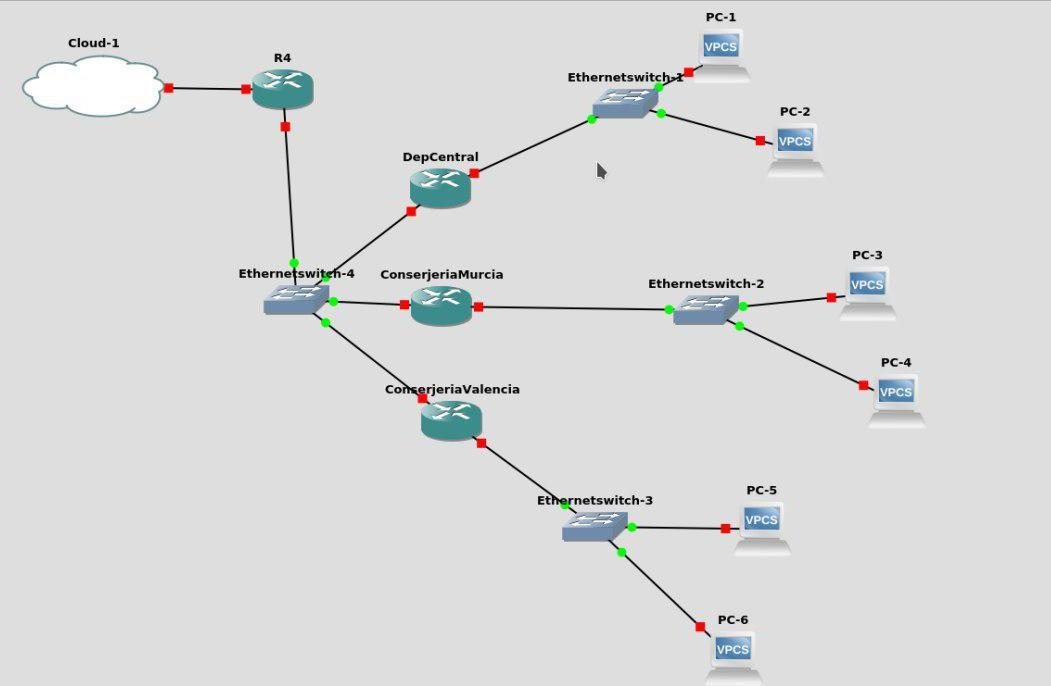
\includegraphics[width=1\textwidth]{topoideal.jpg}
         \caption{Topología ideal.}
         \label{fig:topoideal}
    \end{center}
\end{figure}

\newpage 
%topologia ideal FALTA FOTO Y EXPLICACIÓN
 Una vez presentada la topología ideal, nos centraremos en explicar 

.........

 En la topología se debe desplegar una serie de servicios telemáticos, así como se deberá proteger el acceso a éstos y la transmisión de los paquetes de forma posterior al despliegue.  Concretamente la topología debe incluir los servicios de monitorización de los dispositivos de la red a través del protocolo SNMP, un servicio de almacenamiento de información en la nube mediante el despliegue de owncloud, llamadas sobre voIP para
lo que se llevará a cabo el despliegue del servicio asterisk y un directorio activo para la autenticación en los servicios de owncloud y asterisk mediante LDAP.


 Dados los servicios que se deben desplegar supondremos que serán implementados en las conserjerías de cada gobierno autonómico, en concreto, en la Región de Murcia y la Comunidad Valenciana. Dichas conserjerías estarán gestionadas por un departamento central que se encargará de la administración de red y de solucionar cualquier avería que pueda ocurrir en ambas conserjerías. Se ha elegido este escenario real por la necesidad de almacenamiento en la nube para la disponibilidad de compartición de documentos en la nube o la necesidad de repositorio de almacenamiento para los usuarios de estas organizaciones así como la implementación de una comunicación vía voIP entre las conserjerías y el departamento central para el abaratamiento de coste de las llamadas entre ellos, ya que no se necesita
incurrir en un gasto adicional de líneas telefónicas.


 La organización 110, llamada departamento central, constará de la implementación y despliegue funcional de los servicios de monitorización de red, cloud, voIP y del directorio activo que será utilizado por las dos conserjerías para el acceso al servicio cloud.


 En el caso de las organizaciones 111 y 112, conserjería de Murcia y Valencia respectivamente, se consta del despliegue del servicio de monitorización y de voIP. Para que ambas tengan acceso a los datos de forma conjunta se va a permitir el acceso al servicio cloud desplegado en la organización principal. La centralización de la información supone un riesgo de cara a recibir ataques que comprometan la información que los usuarios transmitirán o solicitarán al cloud con lo que la idea principal será establecer un tunelado IPSec para que dicha información no
se transmita a través de la red en claro. En el caso de asterisk suponemos que la red interna de ambas organizaciones es segura y no requerirá incluir un cifrado de la información transmitida desde el cliente a la centralita y viceversa.


\newpage

\section{Protocolo SNMP}
El protocolo SNMP (Simple Network Management Protocol) consiste en la monitorización de los distintos componentes de una red. Dentro de este protocolo encontramos dos roles posibles, el rol de agente que será el que asume el dispositivo manejado y el de manejador que se encargará de solicitar la información de monitorización al agente.


 En nuestro escenario ideal se ha aplicado la versión 2 de éste protocolo. Hemos decidido esto porque las organizaciones están conectadas entre sí mediante un túnel VPN, por lo que entre ellas solo se generará tráfico interno y no será necesario la securización de SNMP versión 3. 


 La versión 2 del protocolo SNMP se caracteriza por la inclusión de nuevos comandos de interés como getbulk para recuperar información en grandes cantidades y mejora de funcionalidad de la primera versión como en el caso de los trap.


 Los trap son mensajes lanzados por el agente para notificar de situaciones de error o excepcionales, en el caso de la versión 2 lo que se ha hecho ha sido mejorar su función
ya que estaban disponibles en la primera.


 En el caso de la operación getbulk se incluye con el fin de mejorar la obtención de información por parte del manejador ya que, de este modo, puede obtener grandes cantidades de información con una única solicitud, a diferencia de la primera versión.


 Los MIB o Management Information Base, son estructuras jerárquicas que contienen la información de todos los dispositivos gestionados a través de este protocolo. Los arboles de información SNMP constan de dos tipos distintos de nodos: estructurales o de información. Los nodos estructurales no contienen información útil del sistema sino que almacenan su posición en el árbol, son ramas del árbol. En cambio los nodos de información son nodos hoja, estos nodos se basan en la macro object-type que contiene cláusulas para la definición de características de un MIB, es decir, se encargan de definir los tipos de datos de los MIB.


 SNMPv2 se compone de los siguientes nodos estructurales: system, interfaces, at, ip, icmp, tcp, udp, egp y translation.
Del nodo System cuelga información genérica del sistema gestionado como la información de localización o el nombre. 

\subsection{Definición de usuarios}
\subsection{Fichero de configuración}
\subsection{Análisis de trazas}

\newpage
\section{Protocolo de voz sobre IP}

A continuación, vamos a desplegar un servicio de VoIP basado en el uso de Asterisk y SIP en todas las organizaciones.
La VoIP intenta emular a la telefonía tradicional. Mientras que en ésta el envío del audio se realiza de forma analógica a través de unos circuitos virtuales, en la VoIP el audio es enviado digitalmente como paquetes de datos sobre el protocolo IP.


 En una llamada de VoIP diferenciamos las siguientes etapas:
\begin{itemize}
    \item El establecimiento de la llamada que enviará ese audio (SIP).
    \item La conversión del audio analógico en digital (códecs).
    \item El envío de ese audio por la red desde un origen hasta un destino (RTP).

\end{itemize}

\subsection{Protocolo SIP}
El protocolo SIP, Session Iniciation Protocol, es un protocolo de señalización end-to-end. Permite establecer una llamada entre dos usuarios sobre una red IP, negociando las características de la misma. Sin embargo, la función de SIP es únicamente de sincronización, puesto que no transporta audio ni garantiza la calidad del uso de este protocolo de transporte. 


 SIP se encarga de establecer la conexión entre los equipos y de establecer las características que tendrá la llamada, pero no garantiza que la red pueda soportar las características establecidas.
Para implementarlo, los equipos finales implementan dos Agentes SIP diferentes: User Agent Client (UAC), y User Agent Server (UAS). El primero se utiliza para realizar solicitudes de llamadas, es decir, para realizar una llamada. Y el segundo para recibirlas.



Además, se diferencian tres tipos de Servidores:

\begin{itemize}
    \item Por un lado, el Proxy Server y el Redirect Server que se encargan de proporcionar la información necesaria para que la llamada llegue hasta el destinatario (el proxy server redirige la llamada directamente, mientras que el Redirect Proxy indica la IP en la que se encuentra el destinatario).
    
    \item Por otro lado, el Registrer Server acepta solicitudes de registro de usuarios, y mantiene la localización de los mismos en un Servidor de Localización (Location Server). El Registrer Server se puede localizar en la misma máquina que el Proxy/Redirect o en otra distinta. 
    
\end{itemize}  


Todos los terminales se registran, nada más iniciarse, en el Register Server, donde se asocia su ID de usuario con su IP. De esta forma, al realizar una llamada, los proxys buscan la IP del equipo al que queremos llamar, o nos redirigen directamente hacia él (Proxy Server), o nos indica la IP (Redirect Server).
Una vez que ya conocemos la IP del equipo al que queremos llamar, entra en juego el protocolo SIP propiamente dicho. En la figura \ref{fig:1} podemos ver un ejemplo de una negociación básica SIP.

%% mirar pq no me referencia bien la etiqueta
\begin{figure}[htb]
\label{fig:1}
    \begin{center}
        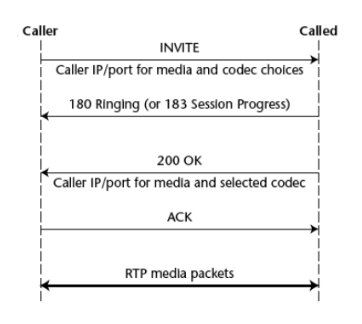
\includegraphics[width=0.7\textwidth]{sip-register.jpg}
         \caption{Negociación básica SIP.}
    \end{center}
\end{figure}

 El mensaje \textit{INVITE} indica la IP y el puerto en los que el llamante quiere que el llamado envíe el audio, así como los códecs y la tasa de muestreo que soporta.


 El receptor de la llamada responde con un \textit{180 Ringing}, esto se reproducirá en el equipo receptor como tono de llamada.

  Tras esto, enviará un mensaje \textit{200 OK}, indicando en qué dirección IP y en qué puerto quiere recibir los datos de la llamada, así como los códecs y la tasa de muestreo seleccionados para la misma. Aquí es importante remarcar que SIP no ofrece QoS (Calidad de Servicio), y por tanto las características
seleccionadas por el receptor podrían no ser soportados por la línea.

 
Finalmente, el llamante envía un mensaje \textit{ACK} dando comienzo así a la transmisión de la llamada mediante el protocolo encargado de ello, que será RTP.

 
Cabe destacar que, si bien el envío de paquetes RTP puede ser directamente entre los dos equipos, los mensajes SIP se envían a través de los servidores proxy.

\subsection{Protocolo RTP}
El protocolo RTP, Real Time Protocol, ofrece entrega extremo a extremo de servicios
en tiempo real. Utilizando, principalmente, UDP como protocolo de transporte.

 
Para el envío, el emisor simplemente coge el fragmento de datos multimedia y le añade una cabecera RTP, encapsula ese paquete en un UDP y añade la cabecera IP. El receptor obtendrá el paquete RTP y transmite el fragmento de datos a la aplicación multimedia.

 
Cabe destacar que RTP no garantiza la entrega ni evita que los fragmentos lleguen fuera de orden. Con el fin de ofrecer información sobre la calidad de la distribución, se utiliza RTCP (Real-Time Control Protocol).

\subsection{Diseño ideal}
A la hora de plantear la implementación y despliegue del servicio voIP en la vida real y no en un escenario ideal, se deben tener en cuenta una serie de factores tales como el hecho de que las organizaciones de nuestro escenario en el mundo real no estarán interconectadas entre sí a través de un router intermedio, sino que tendrán acceso real a la red. Este hecho supone una exposición de los paquetes transmitidos entre centralitas y dispositivos, por lo que se debe tener en cuenta la protección de los paquetes transmitidos y la autenticación de los usuarios.

 
Para llevar a cabo la autenticación de los usuarios se va a seguir un procedimiento estándar basado en nombre de usuario y contraseña que se almacenará en LDAP. 

 
Con respecto a la protección de los paquetes transmitidos durante una llamada y la
negociación de ésta se va a aplicar tunelado IPSec aplicando el protocolo IKE para el intercambio de las claves de cifrado.

  
Dado que en el diseño implementado se ha desactivado la opción de \textit{directmedia},\ref{fig:sip.conf}, el tráfico de las llamadas se transmite entre las centralitas lo que supone una mayor facilidad con respecto a la protección de dicho tráfico. Esto a su vez, supone una mayor exposición y vulnerabilidad de dicho tráfico a posibles ataques.

\subsection{Diseño implementado}

En nuestra escenario hemos desplegado tres centralitas, una en cada organización, encargadas de ofrecer el servicio de telefonía a sus respectivos usuarios. El despliegue de una centralita en la organización que representa al departamento central se ha realizado, ya que hemos visto necesaria la comunicación de las dos conserjerías con el departamento que las administra para comunicar incidencias o consulta de dudas.

 
Para autenticarse, los usuarios utilizan un usuario y contraseña. El administrador de cada organización será el encargado de darlos de alta en la centralita de su organización, y una vez registrados ya podrán utilizar el servicio de VoIP. Esto lo harán autenticándose en uno de los dispositivos de la red habilitados como clientes, en un ordenador utilizando jitsi. En nuestro caso, como tenemos una topología virtualizada no es posible utilizar una app para el teléfono móvil ya que la conexión de dicho teléfono no pertenece a la misma red dónde se encuentran nuestras centralitas desplegadas.

 
Con respecto al paso del tráfico de paquetes RTP, hemos establecido que éste irá a través de las centralitas. Aunque esto provoque un aumento del tráfico entre centralitas, la cantidad de llamadas en espera no supondrá una sobrecarga excesiva para éstas, ya que en principio, este servicio está pensado para comunicación entre los usuarios de las organizaciones internas y no para comunicaciones con el exterior.

 
La principal ventaja de esta decisión es la seguridad, ya que, al ir todo a través de las centralitas, con proteger el tráfico entre ellas nos aseguramos de que todo el tráfico en las llamadas es seguro, así como nos ahorramos el tener que proteger aparte el tráfico RTP entre los dos clientes, lo que supone un aumento del coste de despliegue del servicio. 


 En nuestro caso, no será necesario proteger los canales SIP, ya que nuestras organizaciones están interconectadas entre sí mediante una VPN común, por lo que el tráfico no saldrá de la red interna.

\subsection{Configuración de ficheros}
El administrador de cada organización deberá configurar la información de los usuarios en el fichero \textit{/etc/asterisk/users.conf}. 


\begin{figure}[htb]
    
    \begin{center}
        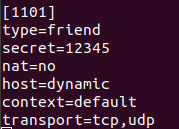
\includegraphics[width=0.4\textwidth]{1101.jpg}
         \caption{Ejemplo de extensión 1101.}
         \label{fig:1101}
    \end{center}
\end{figure}

\newpage
 En la figura \ref{fig:1101} podemos ver la configuración en el fichero \textit{/etc/asterisk/users.conf} de la extensión de un usuario de la organización del departamento central. Este usuario es de tipo friend, ya que queremos que se autentique en las llamadas salientes y entrantes, la contraseña para acceder a su extensión es "12345", el host lo hemos configurado como "dynamic\" ya que se permite que inicie sesión desde una IP dinámica, su contexto es default, ya que en el fichero \textit{/etc/asterisk/extensions.conf} la configuración de esta extensión se encuentra en el contexto [default] y utiliza como protocolo de transporte TCP y UDP.


 Para la comunicación entre usuarios de diferentes organizaciones necesitamos configurar en \textit{/etc/asterisk/users.conf} los troncales de dichas organizaciones para que cuando una centralita reciba una solicitud de llamada para una extensión que no está en su conjunto de extensiones redirija el tráfico a la centralita correspondiente. 


\begin{figure}[htb]
    \begin{center}
        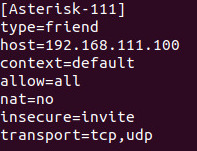
\includegraphics[width=0.4\textwidth]{asterisk-111.jpg}
         \caption{Troncal de la organización de la conserjería de Murcia.}
          \label{fig:a-111}
    \end{center}
\end{figure}

 Como podemos ver en la figura \ref{fig:a-111} [Asterisk-111] es utilizado para realizar la redirección de las llamadas de la Conserjería de Murcia en la organización del departamento central. Esta redirección se establecerá por medio de una extensión en el fichero \textit{/etc/asterisk/extensions.conf}. En el parámetro host se configura la IP donde se aloja la centralita del departamento central y la opción ``insecure=invite'' omite la autenticación en las llamadas entrantes.


 En el fichero \textit{/etc/asterisk/extensions.conf} se especifica   la   lógica   del   plan   de marcado. Define qué hacer con los diferentes tipo de canal y las llamadas entrantes y salientes. En la figura \ref{fig:troncales} podemos observar como se configura la redirección del tráfico hacia otras centralitas. En este caso, en la Conserjería de Valencia se ha configurado que cuando llegue una llamada con extensión 111X o 110X reenvíe el tráfico a las centralitas de la Conserjería de Murcia y del Departamento Central respectivamente.

\begin{figure}[htb]
    \begin{center}
        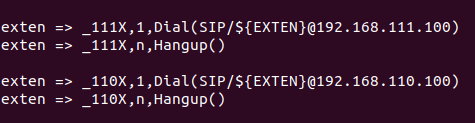
\includegraphics[width=0.9\textwidth]{troncales.png}
         \caption{Redirecciones realizadas en la Conserjería de Valencia.}
         \label{fig:troncales}
    \end{center}

\end{figure}

 Para configurar que todo el tráfico pase por nuestras centralitas como hemos explicado en las secciones anteriores hemos configurado el parámetro ``directmedia=no'' en el fichero \textit{/etc/asterisk/sip.conf} como se muestra en la siguiente figura.

\begin{figure}[htb]
    \begin{center}
        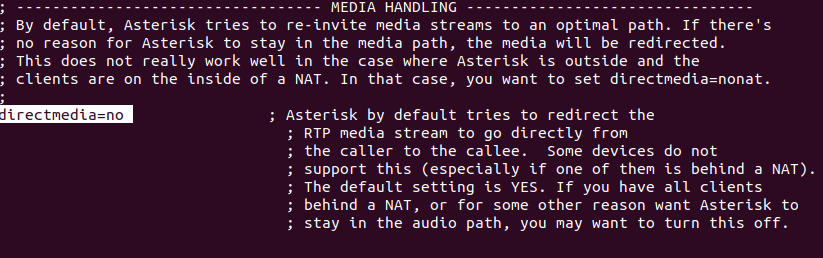
\includegraphics[width=1\textwidth]{sipconf.jpg}
         \caption{/etc/asterisk/sip.conf}
         \label{fig:sip.conf}
    \end{center}
\end{figure}

\subsubsection{Implementación de buzón de voz en los clientes.}

Una de las configuraciones extras que se nos propuso por parte de los profesores de la asignatura es la de la configuración de un buzón de voz para cada usuario de las organizaciones. 


 Esta configuración será bastante útil para los usuarios, ya que cuando un usuario no conteste a los 20 segundos de iniciar el tono de llamada saltará el buzón de voz y esto permitirá guardar mensajes de otros usuarios para poder ser escuchados después por si la llamada era urgente.


 Para ello, se ha configurado en el fichero \textit{/etc/asterisk/voicemail.conf} para cada cliente un buzón, como podemos ver en la figura \ref{fig:voicemail.conf}.

\begin{figure}[htb]
    \begin{center}
        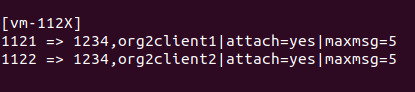
\includegraphics[width=0.8\textwidth]{voicemail.jpg}
         \caption{/etc/asterisk/voicemail.conf}
         \label{fig:voicemail.conf}
    \end{center}
\end{figure}

 El primer atributo define la contraseña de acceso al buzón, seguido del nombre del usuario, el atributo attach con valor ``yes'' nos permite notificar al usuario por correo electrónico de que tiene un mensaje en su buzón y el atributo maxmsg es la cantidad máxima de mensajes que tendrá almacenados el buzón de voz, en este caso será de 5 mensajes no escuchados.


 Una vez definidos los buzones de voz como se ha visto anteriormente, definiremos en el fichero \textit{/etc/asterisk/extensions.conf} cada extensión de usuario, como se muestra en la figura \ref{fig:extensions.conf}.

\newpage
\begin{figure}
    \begin{center}
        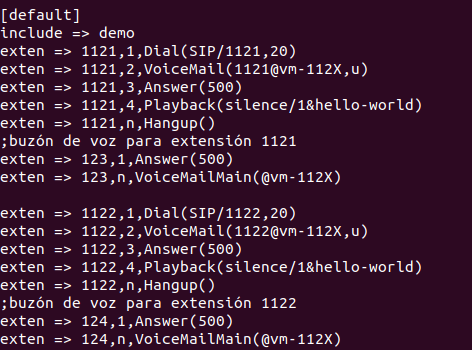
\includegraphics[width=0.8\textwidth]{extens+buzon.png}
         \caption{/etc/asterisk/voicemail.conf}
         \label{fig:extensions.conf}
    \end{center}
\end{figure}

En este caso, mostramos el fichero de configuración de extensiones de la centralita de la Conserjería de Valencia, como hemos explicado anteriormente cuando un usuario no conteste a los 20 segundos de realizar el inicio de la llamada, saltará el buzón de voz. 

  Si contesta la llamada, se establecerá unos segundos de silencio entre los dos interlocutores con la sentencia ``silence'' de Playback, esto se ha establecido así ya que puede ocurrir que no se establezca la llamada a la vez y se pierda audio, por lo que estableciendo esto nos aseguramos de que esto no pase.

 
Para cada buzón de voz se ha configurado una extensión para poder escuchar los mensajes almacenados, en el caso de la extensión ``1121'' llamará a ``123'' para escuchar sus mensajes almacenados introduciendo su extensión y su contraseña.

 
Por último, como podemos ver en la figura \ref{fig:prueba}, el usuario con extensión ``1122'' tiene un mensaje sin escuchar almacenado en su buzón de voz.

\begin{figure}
    \begin{center}
        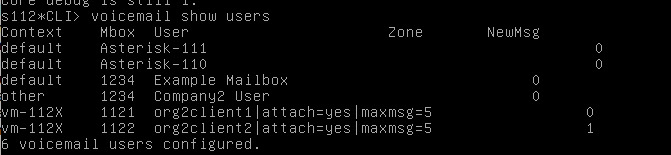
\includegraphics[width=1.1\textwidth]{buzonvoz.jpg}
         \caption{Prueba de correcto funcionamiento.}
         \label{fig:prueba}
    \end{center}
\end{figure}

\newpage
\subsection{Análisis de trazas}
Una solicitud SIP válida debe, como mínimo, contener los siguientes campos:
\begin{itemize}
    \item To: por un lado, especifica el destinatario de la solicitud donde se incluye una, o varias, SIP URI y, por otro lado, un tag que identificará al interlocutor. Cuando se lleva a cabo una solicitud fuera de un dialogo no se incluye el segundo campo.
    \item From: incluye la identidad del dispositivo que inició la solicitud. También incluye el atributo tag, que identificará al interlocutor del diálogo.
    
    \item CSeq: establece una forma de identificar y ordenar transacciones. Está formada por un número de secuencia y un método. Su valor inicial es aleatorio, y se va incrementando con cada solicitud. El método que aparece en esta cabecera coincide con el de la solicitud SIP.
    
    \item Call-ID: actúa como un identificador de sesión, es decir, determina qué mensajes corresponden a un diálogo concreto, tanto en espacio como en tiempo, utilizando un identificador único global. A la hora de generar un Call-ID, la UA que lo genera debe garantizar que ninguna otra generará otro igual, ya que esto podría provocar que se duplicaran los identificadores. Cuando una petición se repite, después de un cierto número de respuestas fallidas, estas respuestas repetidas no se consideran nuevas peticiones y, por tanto, no necesitan nuevos campos Call-ID.
    
    \item Max-Forwards: sirve para limitar el número de saltos proxy que una solicitud puede dar hasta llegar a su destino. Es un entero que se ve reducido en un valor unitario en cada salto. Si su valor llega a 0 antes de llegar a su destino, será rechazado. Por defecto, su valor es 70.
    \item Via indica el transporte utilizado para la transacción así como a dónde debe ser enviada la respuesta, es decir, registra la ruta de la solicitud.
\end{itemize}
\subsubsection{Comunicación entre usuarios de la misma organización}
En una comunicación voz IP, el primer paso es llevar a cabo la autenticación de los usuarios en la centralita, proceso conocido como REGISTER, figura \ref{fig:autenticacion}, aquí se lleva a cabo la asociación de un ID de usuario con su IP. Este identificador se compone de su nombre de usuario seguido del dominio de la organización a la que pertenece. Las trazas analizadas en esta sección se han realizado con la opción ``directmedia=yes'', esto hace que el tráfico RTP se envíe directamente entre los clientes y no tenga que pasar por la centralita y ésta enviarlo a cada usuario. 


\begin{figure}[htb]
    \begin{center}
                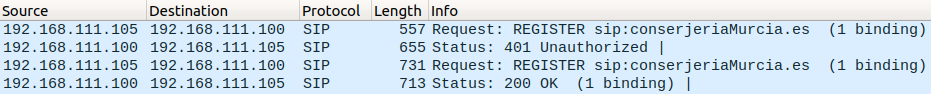
\includegraphics[width=1.1\textwidth]{autenticacion.png}
         \caption{Autenticación de un usuario.}
         \label{fig:autenticacion}
    \end{center}
\end{figure}

 Como podemos ver en la figura \ref{fig:autenticacion}, se quiere realizar un registro en la centralita de la Conserjería de Murcia, en este caso es el usuario con extensión 1111. En el intento de registro el usuario ha recibido un ``401 Unauthorized'', esto ocurre porque en SIP, los usuarios intentan registrarse pero no envían sus credenciales de autenticación a la centralita, por lo que ésta deniega el registro. Una vez recibido la denegación, vuelven a solicitar el registro pero esta vez incluyendo las credenciales de autenticación, y si los datos son correctos, reciben, como en este caso, la confirmación del registro con el mensaje ``200 OK''.
\newpage
\begin{figure}[htb]
    \begin{center}

        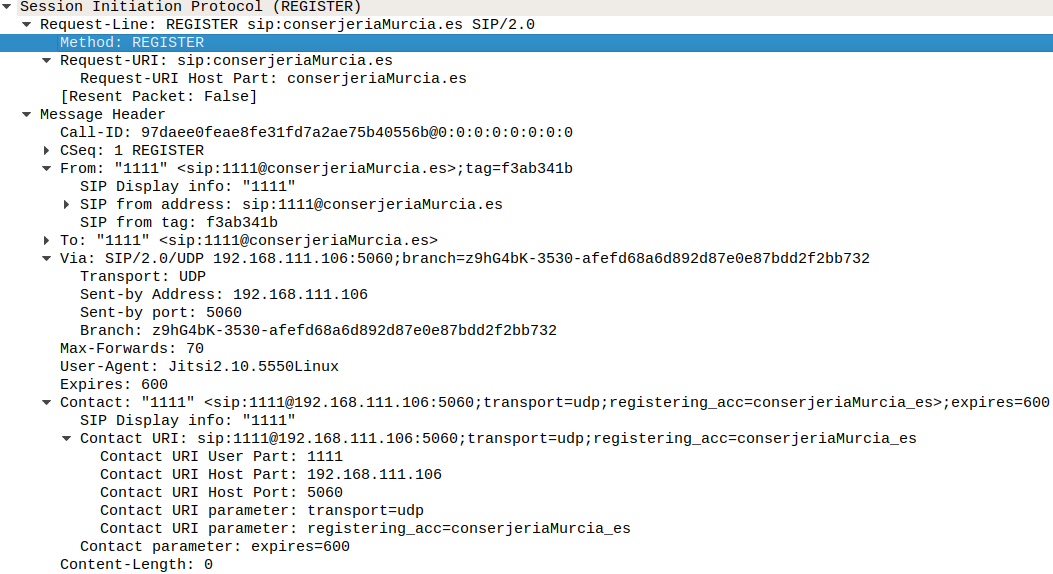
\includegraphics[width=0.9\textwidth]{register1.png}
         \caption{Mensaje Register 1.}
         \label{fig:reg1}
    \end{center}
\end{figure}

 En el primer \textit{Register} enviado, figura \ref{fig:reg1}, podemos ver que el usuario 1112 está intentando registrarse en su centralita como se puede ver en la cabecera ``Contact''.


 El siguiente mensaje, \textit{401 Unauthorized}, es enviado por la centralita al cliente para informarle de que el registro ha fallado. Con la cabecera ``WWW-Authenticate'', mostrada en la figura \ref{fig:401-2} la centralita le indica al cliente los esquemas de autenticación y los parámetros aplicables al URI de solicitud, necesarios para realizar el registro. Con la cabecera ``Nonce Value'' le indica un reto y con ``Algorithm''  nos indica el algoritmo de cifrado que se utilizará para no enviar la contraseña en texto plano.


 El segundo \textit{Register} que envía el UA para realizar el proceso de autenticación tiene los mismos atributos que el primero, pero esta vez sí que incluye los atributos necesarios para realizar la autenticación en la centralita, esto se puede ver en la cabecera ``Authorization''.

 En esta cabecera podemos ver que para autenticarse sigue el método ``Digest access authentication'', que es un método de autenticación muy utilizado para negociar credenciales. En la cabecera ``Digest Authentication Response'' se encuentra la contraseña del usuario cifrada con el algoritmo MD5.

\begin{figure}
    \begin{center}
        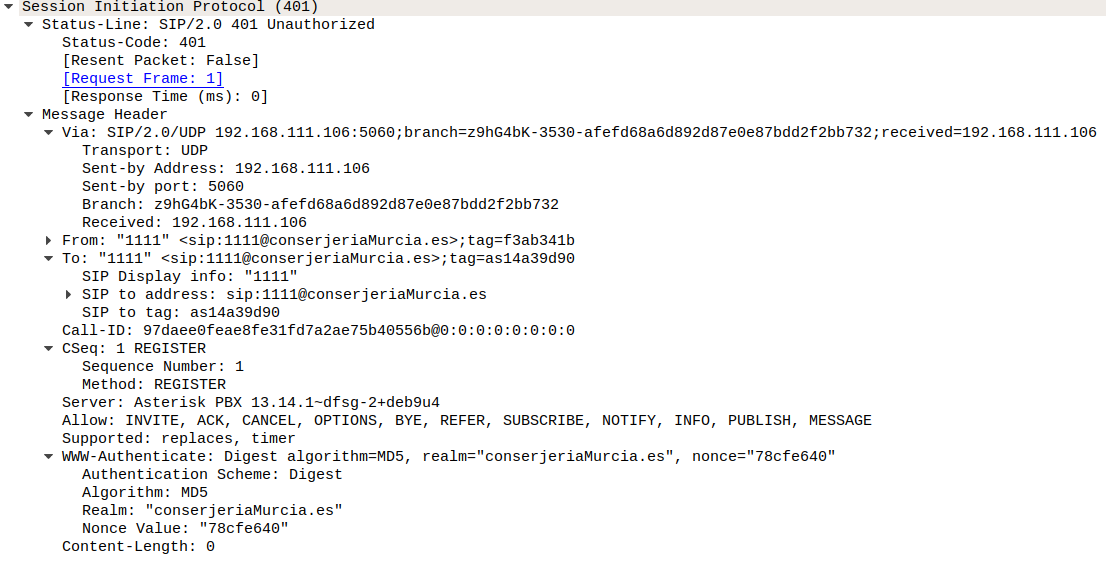
\includegraphics[width=1\textwidth]{401.png}
         \caption{Mensaje 401 Unauthorized.}
         \label{fig:401-2}
    \end{center}
\end{figure}
\begin{figure}
    \begin{center}
        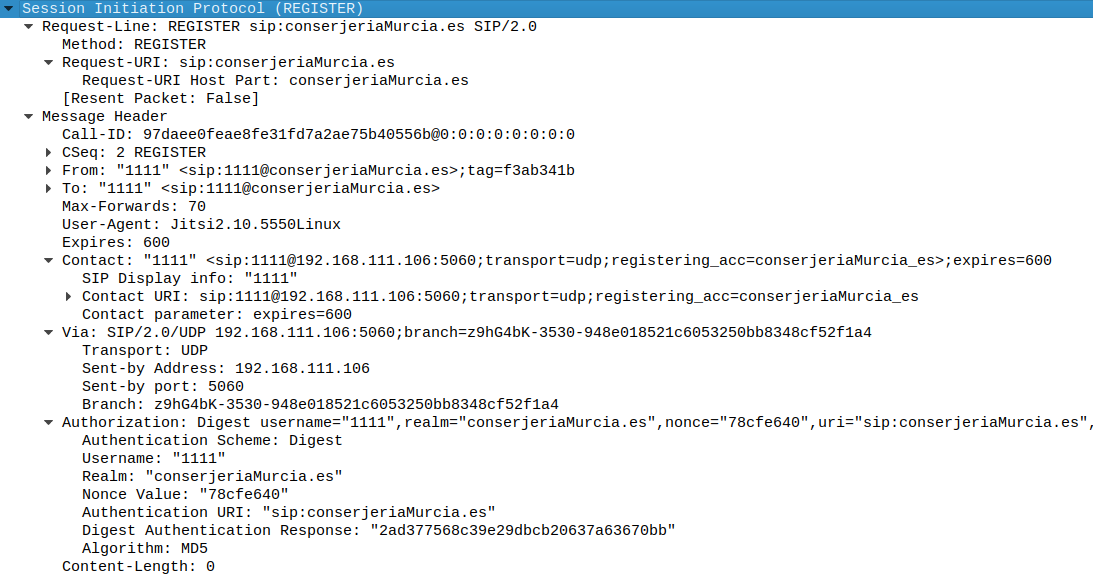
\includegraphics[width=1\textwidth]{register2.png}
         \caption{Mensaje Register + Authorization.}
         \label{fig:reg2}
    \end{center}
\end{figure}

\newpage
 Por último, la centralita envía el mensaje ``200 OK'' para notificarle al cliente que se ha establecido el registro. Una vez realizado el registro el usuario puede comenzar a recibir/realizar llamadas.

\begin{figure}[htb]
    \begin{center}
        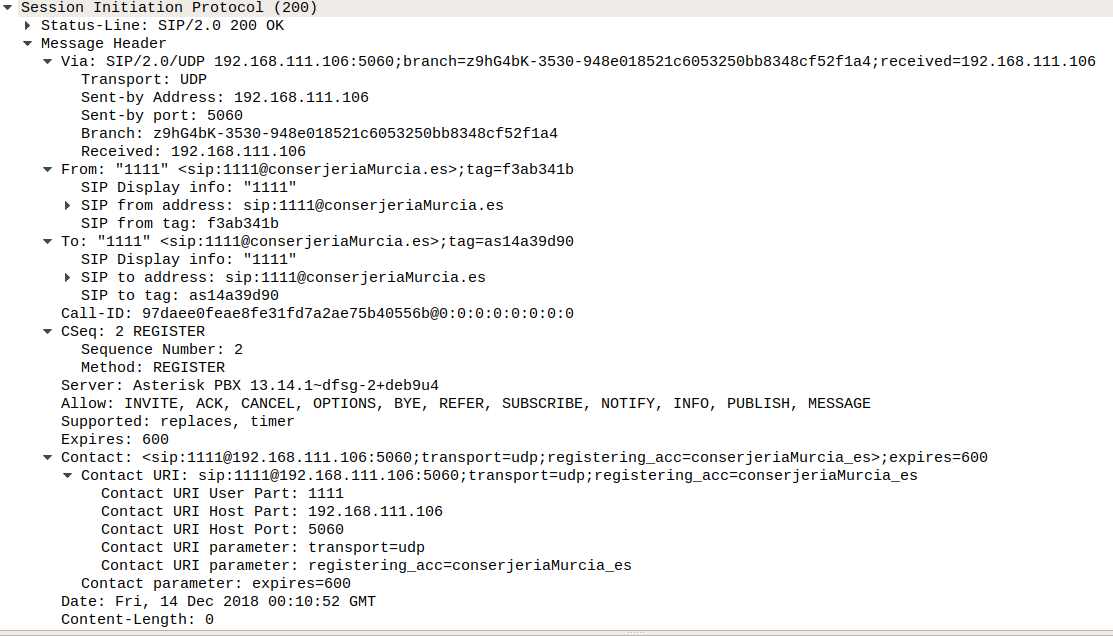
\includegraphics[width=1\textwidth]{200OK.png}
         \caption{Mensaje 200 OK.}
         \label{fig:reg2}
    \end{center}
\end{figure}

 Una vez realizado el proceso de autenticación del usuario, se produce el intercambio de mensajes SIP para llevar a cabo el establecimiento de la llamada. El dispositivo que inicia la llamada envía un mensaje \textit{Invite}, solicitándola e indicando los códecs que soporta. Tras lo que el receptor responde con un \textit{180 Ringing}, indicando que ha podido contactar con el software del teléfono. Finalmente, envía un mensaje \textit{200 OK}, aceptando la llamada e indicando los códecs elegidos de entre los que el llamante indicó. A este mensaje el llamante le responde con un \textit{ACK} con lo que la llamada queda establecida. 

  Una vez explicado esto, mostramos en la figura \ref{fig:establecimiento} una visión general de las trazas capturadas mediante wireshark en la centralita de la Conserjería de Murcia. En la figura \ref{fig:establecimiento} se muestra el proceso de establecimiento de la llamada entre las extensiones 1111 y 1112.

\newpage
\begin{figure}[htb]
    \begin{center}
    
        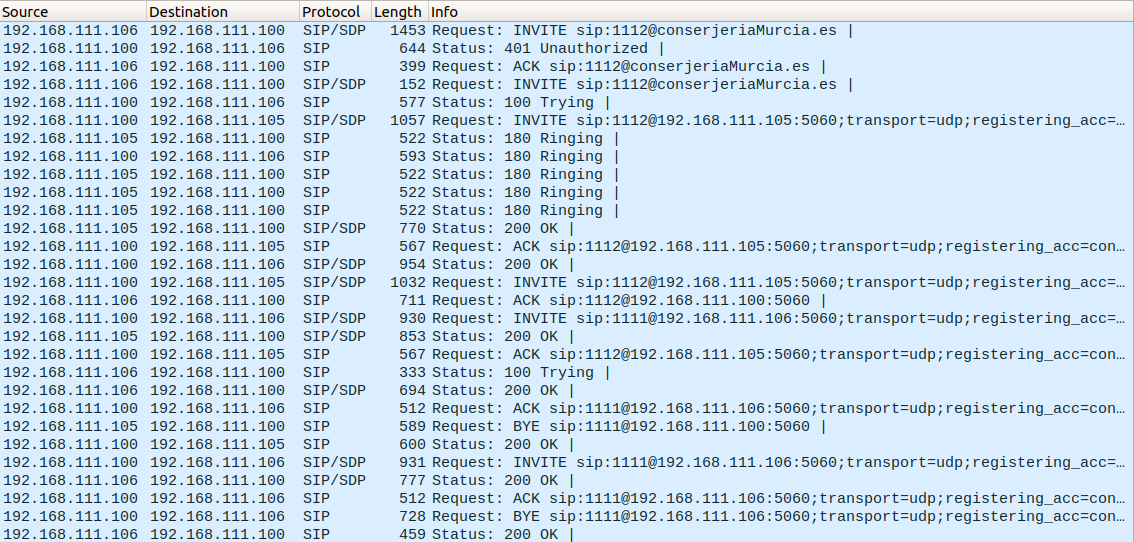
\includegraphics[width=1\textwidth]{esquema-general.png}
         \caption{Trazas de establecimiento de la llamada.}
         \label{fig:establecimiento}
    \end{center}
\end{figure}

  El primer mensaje a analizar es el \textit{invite} que será el encargado de iniciar el proceso de establecimiento de la llamada. Lo envía el dispositivo a través del cual se ha iniciado la llamada, indicando los códecs de audio y/o vídeo que soporta en la misma. En este caso, la llamada se inicia por parte del usuario 1111 desde la centralita de la Conserjería de Murcia, cuya IP es 192.168.111.100 al usuario 1112.

 
 La figura \ref{fig:invite1} contiene la información del mensaje Invite enviado. Como podemos observar, se ha establecido en el campo \textit{Branch} un valor que será el que identifique los paquetes enviados a lo largo de toda la llamada.
\begin{figure}[htb]
    \begin{center}
    
        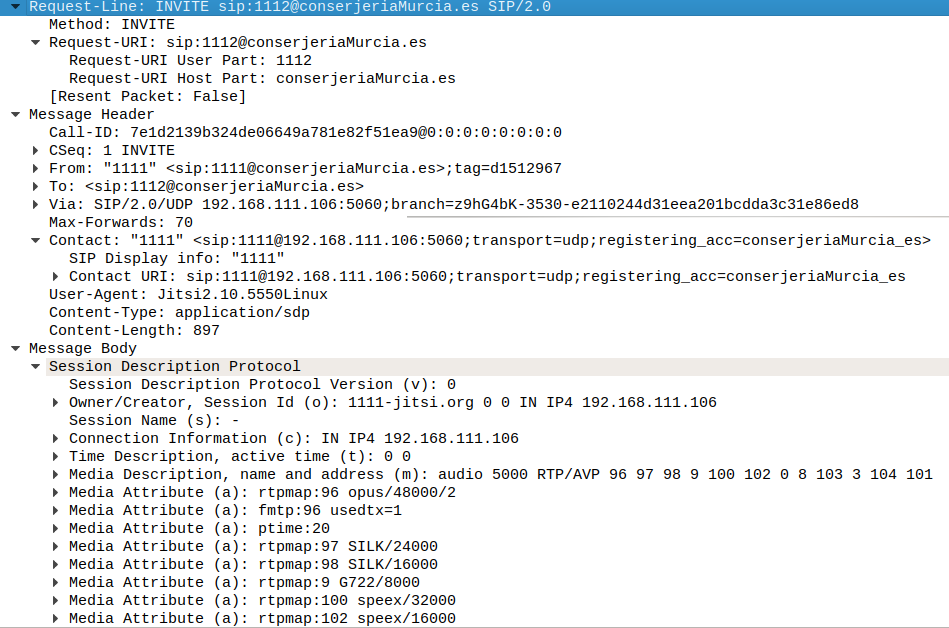
\includegraphics[width=1\textwidth]{invite1.png}
        \caption{Mensaje Invite.}
         \label{fig:invite1}
    \end{center}
\end{figure}

\newpage
 Dentro del contenido del mensaje se puede diferenciar la línea de petición, Request-Line, las cabeceras Message Header y, por último, el cuerpo del mensaje.

 El campo Request-Line será donde se indique el tipo de solicitud, que en este caso es un Invite, así como la Request-URI, es decir, a quién va destinada la petición.

\ En el campo \textit{Via}, podemos observar que se utiliza UDP como protocolo de transporte, que las respuestas deben ir dirigidas a la dirección 192.168.111.105, y el valor del campo Branch puesto que comienza por ``z9hG4bK'' se podrá afirmar que es una rama constituida en base al RFC y, por tanto, única.


\ En la cabecera Message Header, tenemos los siguientes campos: 
\begin{itemize}
    \item  El campo \textit{Call-ID} actúa como un identificador único de la sesión, siendo el mismo para todas las peticiones y respuestas en un diálogo, independientemente de la centralita que las mande.
    \item El campo \textit{CSep} sirve para identificar y ordenar las transacciones, utilizando un método y un número de secuencia. El número de secuencia indica un orden de la solicitud dentro de la conversación.
    \item El campo \textit{From} ofrece el identificador del cliente que ha originado el mensaje, ``sip:1111@conserjeriaMurcia.es''. Puesto que
se trata del comienzo de un diálogo, incluye el campo Tag, que, en este caso, su valor es ``d1512967'', que identifica al interlocutor del diálogo. 

\item En el campo \textit{To} encontramos la especificación del destinatario de la solicitud, en este caso será al cliente:
``sip:1112@conserjeriaMurcia.es''. Puesto que aún no hay un diálogo establecido con ella, el campo Tag no aparece.
\item El campo \textit{Max-Forward} indica el número de saltos proxy que le quedan al paquete para llegar a su destino antes de ser desechado, en el caso de este invite, es 70.
\end{itemize}

En el cuerpo del mensaje se indican los códecs y las tasas de muestreo que el cliente soporta, así como el puerto en el que recibirlos. Como podemos observar, tenemos varias secciones el campo Version no es utilizado por SIP, origin/owner indica el origen de la llamada en
forma de una dirección IP. El campo Media Description indica el formato de la información multimedia, en este caso audio, el puerto al que se envía y los códecs que se permiten utilizar.  Dado que, en este caso, se trata de una llamada, únicamente aparecen códecs de audio. En caso de ser de una videollamada, además de estos aparecería otro Media Description para vídeo, así como sus respectivos códecs. La sección Atribute lista los componentes de cada uno de los códecs indicados en el campo Media Description.


\ El mensaje \textit{401 Unauthorized} es enviado por la centralita para informar al usuario de que la autenticación es requerida. Cabe destacar, que como en la sección anterior, con la cabecera Unauthenticate se informará al usuario del esquema de autenticación utilizado, en este caso ``Digest'' y se le enviará el reto en la cabecera ``Nonce Value'', esto lo podemos ver en la figura \ref{fig:invite-unauthz}.
\newpage
\begin{figure}
    \begin{center}
    
        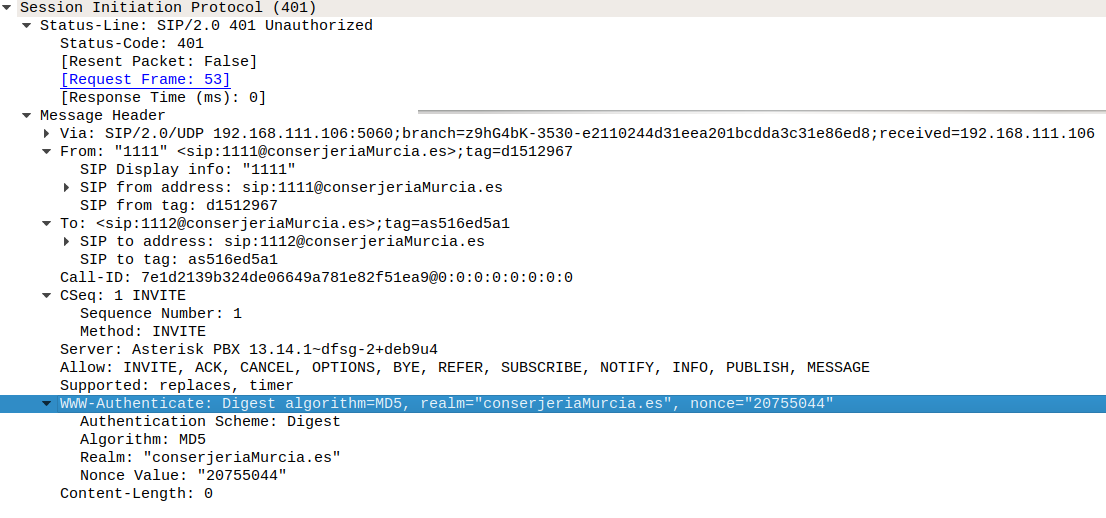
\includegraphics[width=0.8\textwidth]{unauthorized-invite.png}
        \caption{Mensaje 401 Unauthorized}
         \label{fig:invite-unauthz}
    \end{center}
\end{figure}

Cuando el usuario recibe el mensaje \textit{401 Unauthorized} le confirma a la centralita que lo ha recibido con un mensaje ACK y le vuelve a enviar un nuevo Invite, esta vez estableciendo los valores de autenticación solicitados por la centralita, esto se puede ver en la figura \ref{fig:invite-authz}.

\begin{figure}[htb]
    \begin{center}
    
        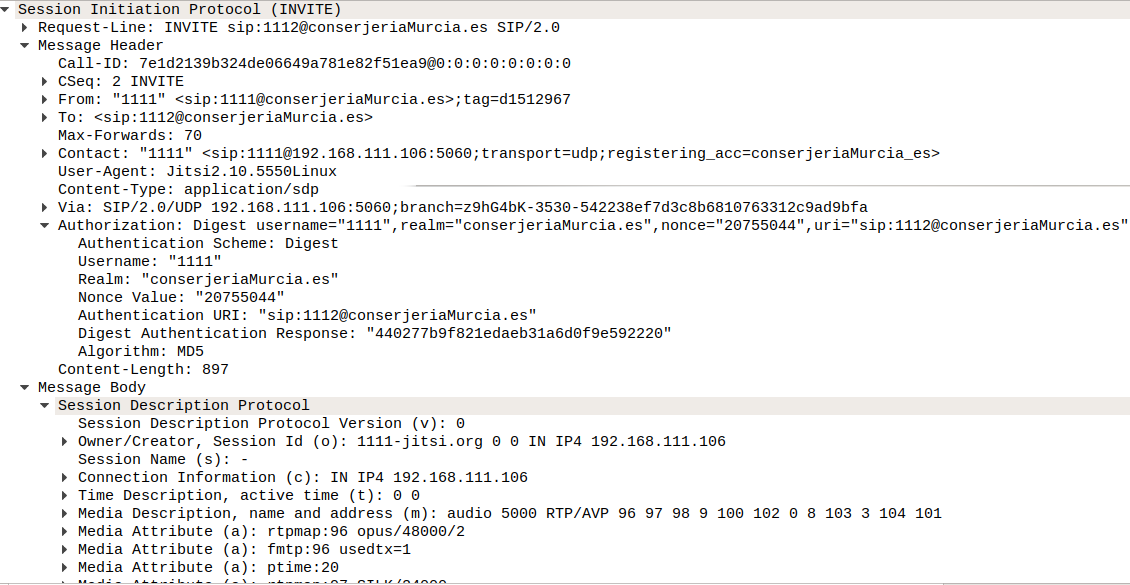
\includegraphics[width=0.85\textwidth]{invite-authz.png}
        \caption{Mensaje Invite + Authentication}
         \label{fig:invite-authz}
    \end{center}
\end{figure}

 El mensaje \textit{100 trying}, figura \ref{fig:trying}, indica que la solicitud ha sido recibida por el servidor y que se está realizando alguna acción relacionada con la llamada. Podemos observar que este mensaje forma parte del mismo dialog, ya que el Call-ID es el mismo que en el mensaje anterior. 
 
También sabemos que responde al mensaje invite previamente enviado puesto que el valor de CSeq se corresponde con 2 INVITE.

\begin{figure}[htb]
    \begin{center}
        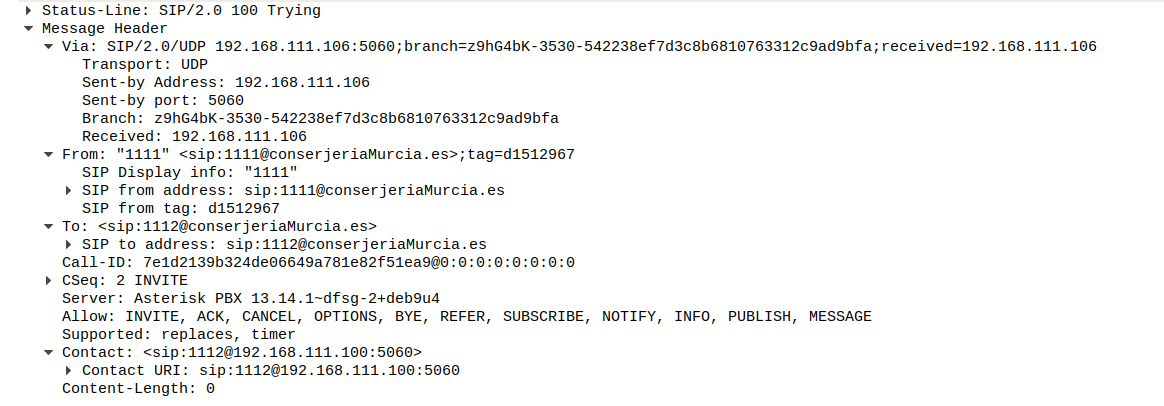
\includegraphics[width=1\textwidth]{100trying_1.png}
        \caption{Mensaje 100 trying.}
         \label{fig:trying}
    \end{center}
\end{figure}

 El mensaje \textit{180 Ringing} indica que la UA que recibió el invite está intentando notificar al usuario. Este mensaje es el que se utiliza para iniciar el tono de llamada. Sabemos que forma parte de esta llamada debido a los valores de CSeq y Call-ID, dado que, como podemos ver en la figura \ref{fig:ring}, son coincidentes con los anteriores valores.
\begin{figure}[htb]
    \begin{center}
        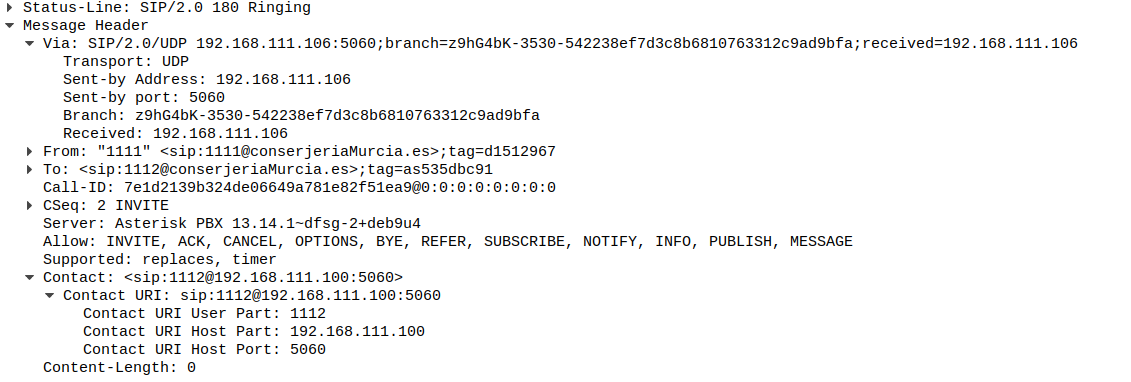
\includegraphics[width=1\textwidth]{180ring.png}
        \caption{Mensaje 180 Ringing.}
         \label{fig:ring}
    \end{center}
\end{figure}

 El mensaje \textit{200 OK} supone la respuesta al Invite aceptando la llamada y con él se indican los códecs seleccionados, así como el puerto en el que desea recibirlos y el ratio de la señal. Cabe destacar que las cabeceras de un mensaje 200 OK son, prácticamente, idénticas a las del mensaje Invite al que confirma, puesto que lo que indican los valores de las cabeceras es información sobre la llamada que se intenta establecer como quién la establece, a quién va dirigida, etc. 
 En Status Line, campo que en el anterior mensaje se denominaba Request-Line, se observa como el mensaje es un mensaje 200 OK, esto se puede ver en la figura \ref{fig:200ok}.
 
\begin{figure}[htb]
    \begin{center}
        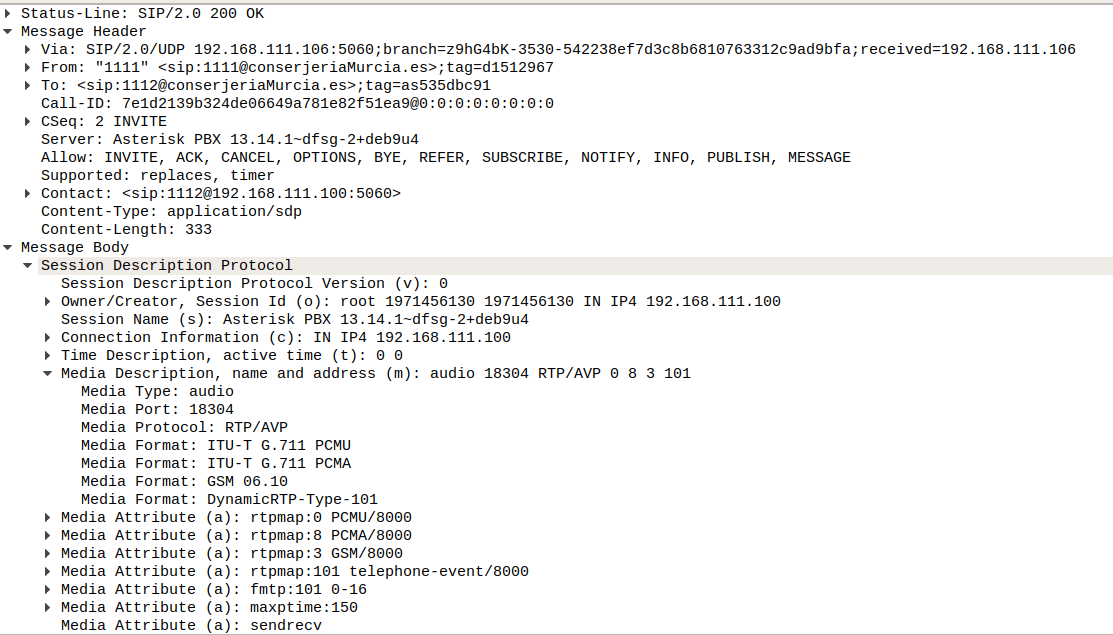
\includegraphics[width=0.8\textwidth]{200OK-2.png}
        \caption{Mensaje 200 OK.}
         \label{fig:200ok}
    \end{center}
\end{figure}

El llamante envía un mensaje ACK confirmando el mensaje anterior. En el campo Request-Line se nos informa de que el mensaje transmitido es un acknowledgement. Los campos Tag, From y To se corresponderán con los anteriores valores.

Cabe destacar, que si la opción ``directmedia=yes'' Asterisk envía INVITES a los dos llamantes para poder enviar paquetes RTP de modo directo, es decir, los paquetes RTP de audio se enviarán directamente entre los llamantes sin pasar por la centralita. Este proceso lo podemos ver en la figura \ref{invitesss}.

\begin{figure}[htb]
    \begin{center}
        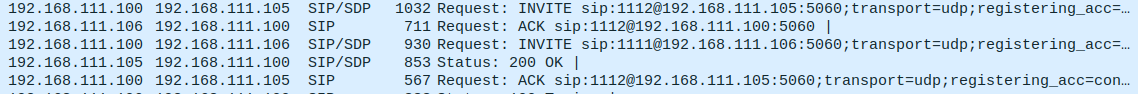
\includegraphics[width=1\textwidth]{invitesRTP.png}
        \caption{INVITES enviados por la centralita}
         \label{fig:invitesss}
    \end{center}
\end{figure}

\newpage
Después de esta confirmación, se ha establecido la llamada y se empiezan a transmitir tráfico RTP, en este caso, en la figura \ref{fig:RTPaudio} tenemos el primer paquete RTP de audio transmitido que, como podemos observar, su contenido ha sido codificado con uno de los códecs negociados durante la aplicación del protocolo SIP.
\begin{figure}[htb]
    \begin{center}
        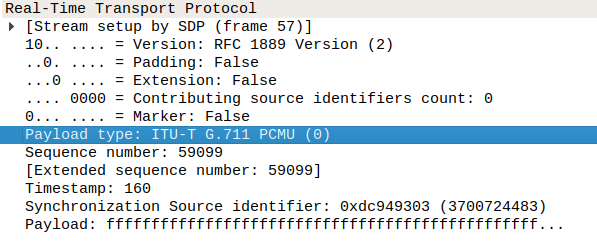
\includegraphics[width=0.6\textwidth]{RTP-1.png}
        \caption{Paquete RTP de audio.}
         \label{fig:RTPaudio}
    \end{center}
\end{figure}

Para finalizar la llamada, el usuario que cuelga envía un mensaje BYE a la centralita y èsta le contesta con un "200 OK". Para que el otro extremo de la llamada sea consciente de que la llamada ha terminado, la centralita le envía un mensaje BYE. Este proceso lo podemos ver en la figura \ref{fig:byess}.

\begin{figure}[htb]
    \begin{center}
        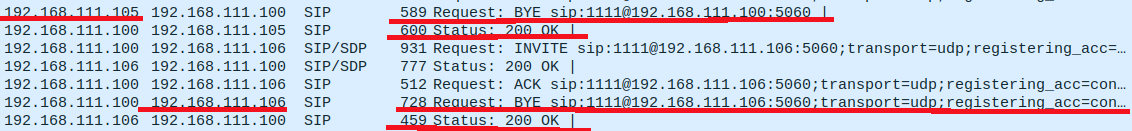
\includegraphics[width=0.9\textwidth]{byes.png}
        \caption{Finalización de la llamada.}
         \label{fig:byess}
    \end{center}
\end{figure}

\newpage
\subsubsection{Comunicación entre usuarios de dos organizaciones distintas}
En esta sección hemos tomado las trazas desde la centralita del Departamento Central y con la opción ``directmedia=no'', esto hará que todo el tráfico de la llamada tanto el tráfico SIP como el tráfico RTP pase por la centralita y sea ella quien lo distribuya como se debe. Cabe destacar que estas trazas se han realizado sin utilizar los dominios de las organizaciones ya que se hicieron antes de establecer la configuración DNS de nuestro escenario. Como se puede ver en la figura \ref{fig:register2}, se realiza el proceso de autenticación del usuario con extensión 1101 en la centralita del Departamento Central.


\begin{figure}[htb]
    \begin{center}
        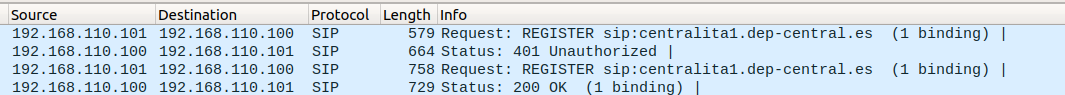
\includegraphics[width=0.9\textwidth]{1112-1101.png}
        \caption{Autenticación extensión 1101.}
         \label{fig:register2}
    \end{center}
\end{figure}


 En la figura \ref{fig:aut2} podemos ver el intercambio de mensajes realizado en el establecimiento de llamada entre el usuario con extensión 1101 y el usuario con extensión 1112 perteneciente a la organización de la Conserjería de Murcia. 

\begin{figure}[htb]
    \begin{center}
        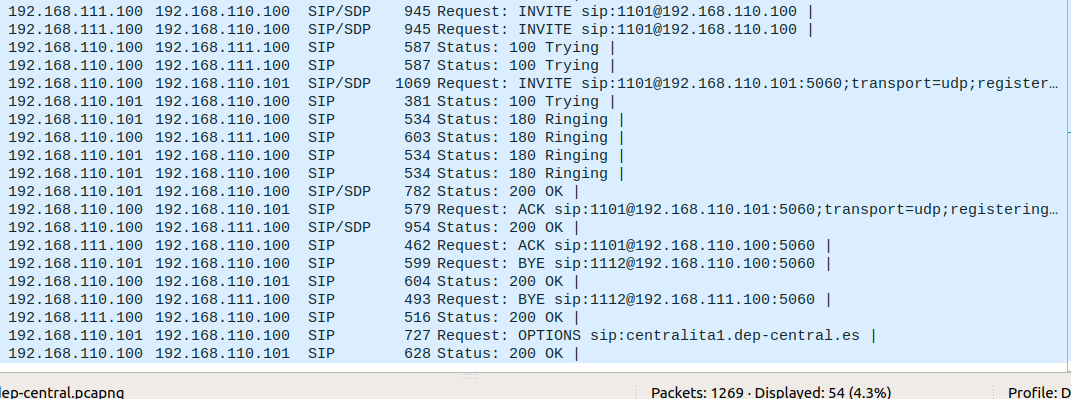
\includegraphics[width=0.9\textwidth]{invite1112-1101.png}
        \caption{Establecimiento de la llamada.}
         \label{fig:aut2}
    \end{center}
\end{figure}

El intercambio de mensajes es muy similar al descrito en en la sección anterior. Con un Invite se inicia el establecimiento de llamada, se recibe un trying para confirmar que la solicitud ha sido recibida y un ringing para informar que se está realizando la llamada. Por último, se establece la llamada con un 200 OK ya que es la confirmación que se recibe para empezar a recibir audio mediante RTP y se finaliza la llamada mediante el mensaje BYE.

\newpage

\section{Servicio Owncloud y LDAP}
\subsection{Diseño ideal}
En el diseño ideal de la topología, todas las organizaciones dispondrán de un servicio centralizado de Owncloud, decimos centralizado porque este servicio de almacenamiento estará alojado en el Departamento Central de nuestro escenario.

En el caso del directorio activo, cada organización tendrá su propio LDAP y será gestionado por el administrador de red.

Este servicio cloud ofrecerá a cada usuario 30 GB de almacenamiento, siendo
ampliable en caso de ser necesario.Esta tarea deberá de ser comunicada al administrador,
quién la llevaría a cabo.

Respecto a los certificados necesarios para el servidor, en nuestro diseño ideal
obtendríamos nuestros certificados de la FNMT-RCM, ya que es el Prestador de Servicios de Certificación utilizado por la administración pública. Esto lo hemos decidido así con el fin de no provocar alarma entre los usuarios por las conexiones no seguras, ya que cuando una conexión no es segura se muestra en el navegador el mensaje de Conexión insegura. Aun así, como en
esta organización todos los trabajadores tendrían un certificado,  dispondríamos de una CA en nuestra organización para proporcionarles nosotros mismos dichos certificados. La CA se encontraría en un equipo del Departamento Central con acceso restringido.

\subsection{Diseño implementado}
En el diseño real implementado, se ha llevado a cabo la inclusión de un único servicio
de owncloud y un solo servicio LDAP para ambas organizaciones. Todas las organizaciones tendrán accesos personalizados al servicio cloud, esto será configurado por los administradores del Departamento Central ya que es allí donde se alojarán en la misma máquina virtual por temas de optimización de recursos. 

\newpage Por este mismo motivo no ha sido necesario cifrar el canal entre ambos, ya
que al encontrarse dentro de la misma máquina se comunican de forma interna.

Los usuarios de nuestro servicio en la nube son dados de alta por el administrador en el
servidor LDAP, de forma que, desde ese instante, ya tienen su cuenta de owncloud
disponible. 

Cada usuario, inicialmente, podrá disponer en ella de hasta 1GB de almacenamiento. Esto puede apliarse si se necesita, realizando una previa solicitud al administrador y siempre teniendo en cuenta el límite establecido por los administradores.

Por simplicidad, tenemos una CA alojada en la misma máquina virtual de LDAP y owncloud, dicha CA estará firmada por la FNMT. Además, dadas las actividades y trámites que realizan los usuarios de nuestras organizaciones cada uno tendrá un certificado cliente propio y accederá a los servicios de su organización autenticándose utilizando su usuario y contraseña, que previamente habrá sido configurado y almacenado en el LDAP central.

\subsection{Directorio activo, LDAP}
El servidor LDAP almacenará información sobre los usuarios de la organización, como
por ejemplo su unidad organizativa, nombre de usuario y contraseña. 

 El servidor de owncloud hará uso de este servidor para realizar la autenticación de los
usuarios en cada solicitud de acceso. Para instalar el servidor LDAP se utilizará slapd y ldap-utils. Una vez introducidos los datos de configuración, se creará un fichero ldif en el que las se insertarán las entradas. 
\subsubsection{Integración de LDAP con Asterisk}
\subsubsection{Análisis de trazas}

\subsection{Servicio Owncloud}
\subsubsection{Integración con LDAP}
\subsubsection{Cuotas de disco de usuarios}
\subsubsection{Establecimiento de conexión segura}
\subsubsection{Revocación de certificados}


\section{Bibliografía}
%----------------------------------------------------------------------------------------
%	BIBLIOGRAFÍA
%----------------------------------------------------------------------------------------
%\backmatter
\nocite{*}
\bibliographystyle{plain}
\bibliography{bibliografía.bib} %Aquí ponen el nombre del archivo .bib






\end{document}